\documentclass{beamer}
\usetheme{metropolis}
\usepackage{graphicx}
\usepackage{subfig}
\usepackage{tcolorbox}
\title{Algebra-Based Physics-2: Electricity, Magnetism, and Modern Physics (PHYS135B-01): Unit 5}
\author{Jordan Hanson}
\institute{Whittier College Department of Physics and Astronomy}

\begin{document}
\maketitle

\section{Unit 4 Review}

\begin{frame}{Unit 4 Summary}
\textbf{Reading: Chapter 22}
\begin{enumerate}
\item Magnets and magnetic fields
\item Force on a moving charge in a magnetic field
\item \textbf{The Hall effect}
\item Magnetic forces on conductors
\item \alert{Amp\`{e}re's Law}
\end{enumerate}
\end{frame}

\section{Summary}

\begin{frame}{Summary}
\begin{enumerate}
\item Maxwell's Equations and Electromagnetic Waves
\item Electromagnetic wave production
\item The Electromagnetic spectrum
\item Waves and Energy
\end{enumerate}
\end{frame}

\section{JITT}

\begin{frame}{JITT}
\textbf{The direction of the electric field shown in each part of Figure 24.5 is that produced by the charge distribution in the wire.  Justify the direction shown in each part, using the Coulomb force law and the definition of $\vec{E} = \vec{F}/q$, where $q$ is positive.}
\end{frame}

\begin{frame}{JITT}
In A, the positive charge is at the bottom and the negative charge is at the top (field has to be upward). In B, the distance between the two charges is zero (no question of direction because the distance becomes zero with the electric field). In C, the distance between the charges is the same as it was in part A but positive charge placed in the downward direction will experience a force that will push it downward. In D, the upward direction is justified (similar to A). 
\end{frame}

\begin{frame}{JITT}
\textbf{Is the direction of the magnetic field shown in Figure 24.6 (a) consistent with the right-hand rule for current (RHR-2) in the
direction shown in the figure?}
\end{frame}

\begin{frame}{JITT}
In (a), using the Right Hand Rule, our thumb points in the course of current. In this case current is upward, so the direction of B should be counter clockwise, which is the direction of our fingers. This appears to be consistent. 
\end{frame}

\begin{frame}{JITT}
Yes, the direction of the magnetic field shown in figure 24.6 is consistent with the right hand rule because a straight up and down wire creates a circular magnetic field around the wire to the right. 
\end{frame}

\begin{frame}{JITT}
\textbf{Why is the direction of the current shown in each part of Figure 24.6 opposite to the electric field produced by the wire’s
charge separation?}
\end{frame}

\begin{frame}{JITT}
The direction of the current is opposite to the electric field because the magnetic field varies with current and propagates away from the antenna at the speed of light, and they are perpendicular to one another and to the direction of propagation.
\end{frame}

\begin{frame}{JITT}
Electric field direction runs in direction of positive test charge, therefore the negative current is in the opposite direction.
\end{frame}

\begin{frame}{JITT}
The current is going upwards at that moment, so it is causing the pos. charge to flow in its own direction, while the neg. charge is going to opposite direction.
\end{frame}

\begin{frame}{JITT}
\textbf{In which situation shown in Figure 24.24 will the electromagnetic wave be more successful in inducing a current in the wire? Explain.}
\end{frame}

\begin{frame}{JITT}
B because the electric field ( E ) shown surrounding the wire is produced by the charge distribution on the wire and the The stronger the E -field created by a separation of charge, the greater the current and, hence, the greater the B -field created.
\end{frame}

\begin{frame}{JITT}
The wire is at rest, so the magnetic field will not induce any current in the wire. Option A will be more successful because we know that an electromagnetic wave consists of electric and magnetic charges. Option A will be more successful due to the directions of the wave which promote waves success. 
\end{frame}

\begin{frame}{JITT}
A because they are perpendicular to one another and create a transverse wave.
\end{frame}

\section{Maxwell's Equations and Electromagnetic Waves}

\begin{frame}{Maxwell's Equations and Electromagnetic Waves}
What is the value $1/\sqrt{\mu_0 \epsilon_0}$?  Do you recognize this value?
\begin{itemize}
\item A: $3 \times 10^{7}$ m/s
\item B: $3 \times 10^{6}$ m/s
\item C: $3 \times 10^{5}$ m/s
\item D: $3 \times 10^{8}$ m/s
\end{itemize}
\end{frame}

\begin{frame}{Maxwell's Equations and Electromagnetic Waves}
\begin{figure}
\centering
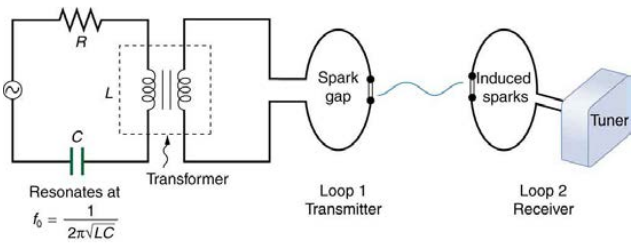
\includegraphics[width=0.5\textwidth]{figures/hertz.png}
\caption{\label{fig:hertz} The apparatus used by Hertz in 1887 to generate and detect electromagnetic waves.  The circuit creates sparks, but also sparks are observed in a different, unconnected circuit.}
\end{figure}
\end{frame}

\begin{frame}{Maxwell's Equations and Electromagnetic Waves}
Hertz also measured the \textit{speed} of the waves using the following equation:
\begin{equation}
v = f \lambda
\end{equation}
\begin{itemize}
\item v is the speed
\item f is the frequency
\item $\lambda$ is the wavelength
\item The inverse of the frequency is the period, $1/f = T$.
\end{itemize}
\end{frame}

\begin{frame}{Maxwell's Equations and Electromagnetic Waves}
The frequency of waves on the shore is 0.2 Hz, and the wavelength is 10 m.  What is the speed with which they approach the shore?
\begin{itemize}
\item A: 1 m/s
\item B: 2 m/s
\item C: 5 m/s
\item D: 10 m/s
\end{itemize}
\end{frame}

\begin{frame}{Maxwell's Equations and Electromagnetic Waves}
The frequency of waves on the shore is 0.2 Hz, and the wavelength is 10 m.  What is the period of the waves?
\begin{itemize}
\item A: 1 s
\item B: 5 s
\item C: 5 m/s
\item D: 10 Hz
\end{itemize}
\end{frame}

\begin{frame}{Maxwell's Equations and Electromagnetic Waves}
The FM radio station 97.9 corresponds to a frequency of 97.9 MHz.  If the speed of light is $3 \times 10^{8}$ m/s, what is the wavelength of the radio station?
\begin{itemize}
\item A: 1 m
\item B: 0.1 m
\item C: 3 m
\item D: 0.3 m
\end{itemize}
\end{frame}

\begin{frame}{Maxwell's Equations and Electromagnetic Waves}
The AM radio station 740 corresponds to a frequency of 740 kHz.  If the speed of light is $3 \times 10^{8}$ m/s, what is the wavelength of the radio station?
\begin{itemize}
\item A: 10 m
\item B: 40 m
\item C: 100 m
\item D: 400 m
\end{itemize}
\end{frame}

\begin{frame}{Maxwell's Equations and Electromagnetic Waves}
A radio wave is observed to propagate through 1000 m of ice in 6 $\mu$s.  What is the speed of the radio wave?
\begin{itemize}
\item A: $3 \times 10^8$ m/s
\item B: $1.67 \times 10^8$ m/s
\item C: $5.4 \times 10^8$ m/s
\item D: $2 \times 10^8$ m/s
\end{itemize}
\end{frame}

\begin{frame}{Maxwell's Equations and Electromagnetic Waves}
Why does is the wave observed to travel slower than the speed of light given by $1/\sqrt{\mu_0 \epsilon_0}$? \\ \vspace{0.5cm}
\begin{equation}
v = c/n
\end{equation}
The index of refraction $n$ changes the wave speed.  The index is always $n > 1$.
\end{frame}

\begin{frame}{Maxwell's Equations and Electromagnetic Waves}
\begin{figure}
\centering
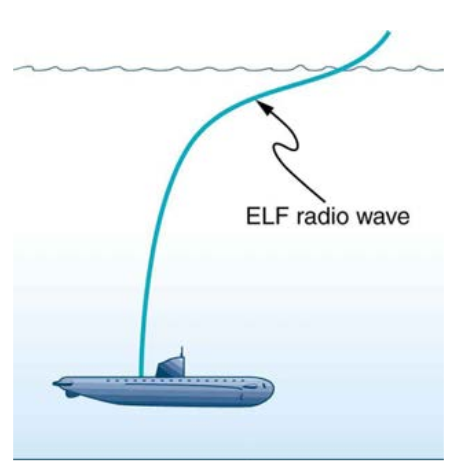
\includegraphics[width=0.5\textwidth]{figures/sub.png}
\caption{\label{fig:sub} Submarines can actually communicate electromagnetically if the frequency is low enough.  Why does the path of light bend?}
\end{figure}
\textbf{Observe example on board, Snell's Law.}
\end{frame}

\begin{frame}{Maxwell's Equations and Electromagnetic Waves}
In the previous figure, which of the following is true of the \textit{index of refraction?}
\begin{itemize}
\item A: It is smaller at the top of the ocean than at the bottom near the sub.
\item B: It is larger at the top of the ocean than at the bottom near the sub.
\item C: It is unform throughout the ocean, at the top and near the sub.
\item D: It is 1 because the ray is traveling approximately straight near the sub.
\end{itemize}
\end{frame}

\begin{frame}{Maxwell's Equations and Electromagnetic Waves}
\textit{A little bit of optics:} \textbf{Snell's Law}
\begin{equation}
n_1 \sin\theta_1 = n_2 \sin\theta_2
\end{equation}
\begin{itemize}
\item $n_1$ is the index of medium 1
\item $n_2$ is the index of medium 2
\item $theta_1$ and $\theta_2$ are the angles with respect to vertical.
\end{itemize}
\end{frame}

\begin{frame}{Maxwell's Equations and Electromagnetic Waves}
A radio wave enters the ocean at a 45 degree angle with respect to vertical.  The index of refraction of water is $n = 1.33$, and the index of air is 1.  What is the new angle of the radio wave with respect to vertical?
\begin{itemize}
\item A: 0 degrees
\item B: 10 degrees
\item C: 20 degrees
\item D: 30 degrees
\end{itemize}
\end{frame}

\begin{frame}{Maxwell's Equations and Electromagnetic Waves}
PhET simulation on the speed of light in materials:
\url{https://phet.colorado.edu/sims/html/bending-light/latest/bending-light_en.html}
\begin{enumerate}
\item Measure the index of refraction of mystery material 1
\item Measure the index of refraction of mystery material 2
\end{enumerate}
\end{frame}

\begin{frame}{Maxwell's Equations and Electromagnetic Waves}
Examine the following function:
\begin{equation}
\vec{E}(t) = E_0 \sin\left(k x - \omega t\right) \hat{k}
\end{equation}
\textbf{Work some examples with this function.}
\begin{itemize}
\item $c/n = f \lambda$
\item $k = \frac{2\pi}{\lambda} = \frac{\omega}{(c/n)}$
\item $\omega = 2\pi f$
\item Euler's formula
\item Graph
\end{itemize}
\end{frame}

\begin{frame}{Maxwell's Equations and Electromagnetic Waves}
Power per unit area in electromagnetic radiation:
\begin{equation}
I_{ave} = \frac{c\epsilon_0 E_0^2}{2}
\end{equation}
\textbf{Example on board, then group board exercise.}
\begin{equation}
Q = m c \Delta T
\end{equation}
(Heat capacity equation).
\end{frame}

\section{Conclusion}

\section{Answers}

\begin{frame}{Answers}
\tiny
\begin{columns}[T]
\begin{column}{0.5\textwidth}
\begin{itemize}
\item $3 \times 10^{8}$ m/s
\item 2 m/s
\item 5 s
\item 3 m
\item It is smaller at the top of the ocean than at the bottom near the sub.
\end{itemize}
\end{column}
\begin{column}{0.5\textwidth}
\begin{itemize}
\item 
\end{itemize}
\end{column}
\end{columns}
\end{frame}

\end{document}
